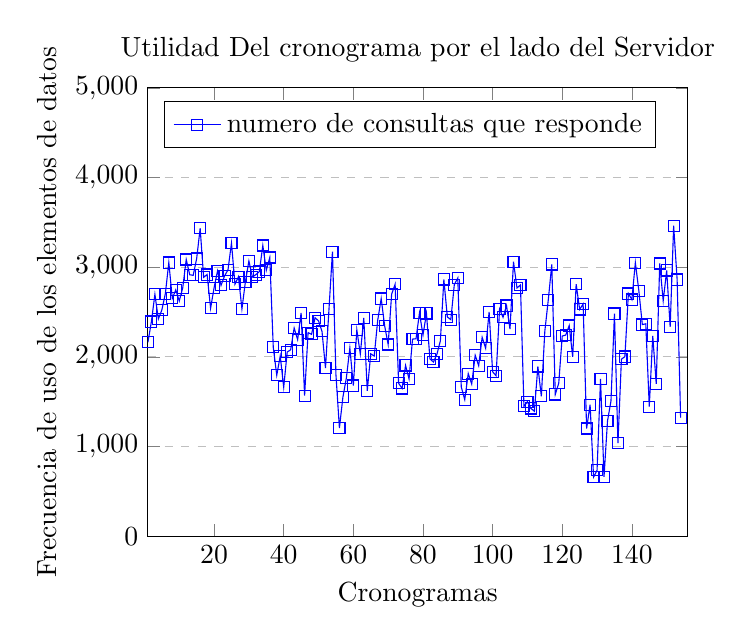
\begin{tikzpicture}
\begin{axis}[
    title={Utilidad Del cronograma por el lado del Servidor},
    xlabel={Cronogramas},
    ylabel={Frecuencia de uso de los elementos de datos},
    xmin=1, xmax=156,
    ymin=0, ymax=5000,
    xtick={},
    ytick={},
    legend pos=north west,
    ymajorgrids=true,
    grid style=dashed,
]

\addplot[
    color=blue,
    mark=square,
    ]
    coordinates {
%UTILIDAD TOTAL
(1,2163)
(2,2394)
(3,2697)
(4,2423)
(5,2523)
(6,2704)
(7,3052)
(8,2652)
(9,2747)
(10,2623)
(11,2770)
(12,3086)
(13,2916)
(14,2909)
(15,3096)
(16,3434)
(17,2887)
(18,2918)
(19,2542)
(20,2770)
(21,2959)
(22,2797)
(23,2901)
(24,2972)
(25,3269)
(26,2810)
(27,2893)
(28,2535)
(29,2838)
(30,3069)
(31,2890)
(32,2917)
(33,2951)
(34,3242)
(35,2966)
(36,3108)
(37,2107)
(38,1795)
(39,2009)
(40,1661)
(41,2053)
(42,2079)
(43,2322)
(44,2192)
(45,2491)
(46,1568)
(47,2270)
(48,2251)
(49,2436)
(50,2402)
(51,2284)
(52,1875)
(53,2530)
(54,3174)
(55,1802)
(56,1207)
(57,1550)
(58,1765)
(59,2100)
(60,1680)
(61,2301)
(62,2032)
(63,2434)
(64,1622)
(65,2034)
(66,2009)
(67,2408)
(68,2650)
(69,2344)
(70,2138)
(71,2699)
(72,2810)
(73,1706)
(74,1648)
(75,1904)
(76,1753)
(77,2198)
(78,2202)
(79,2491)
(80,2243)
(81,2484)
(82,1977)
(83,1942)
(84,2028)
(85,2179)
(86,2863)
(87,2445)
(88,2415)
(89,2805)
(90,2879)
(91,1664)
(92,1523)
(93,1813)
(94,1697)
(95,2017)
(96,1902)
(97,2218)
(98,2096)
(99,2501)
(100,1834)
(101,1790)
(102,2533)
(103,2441)
(104,2572)
(105,2309)
(106,3061)
(107,2768)
(108,2802)
(109,1448)
(110,1500)
(111,1425)
(112,1393)
(113,1893)
(114,1559)
(115,2287)
(116,2638)
(117,3031)
(118,1581)
(119,1707)
(120,2232)
(121,2243)
(122,2349)
(123,2001)
(124,2811)
(125,2529)
(126,2589)
(127,1201)
(128,1467)
(129,659)
(130,734)
(131,1753)
(132,661)
(133,1284)
(134,1508)
(135,2483)
(136,1037)
(137,1974)
(138,2003)
(139,2706)
(140,2639)
(141,3050)
(142,2739)
(143,2360)
(144,2369)
(145,1445)
(146,2234)
(147,1699)
(148,3041)
(149,2625)
(150,2964)
(151,2334)
(152,3462)
(153,2862)
(154,1321)
    };
    \legend{numero de consultas que responde}

\end{axis}
\end{tikzpicture}

